\section{Descripción de circuito con diferentes operadores de asignación \label{sec:s1}}

\begin{center}
	\begin{minipage}{12cm}
		\begin{tcolorbox}[title=Actividad 1]
			Capturar el código de la lámina 7 de la presentación de clase (Asignación en verilog (6)). Compilar y observar el resultado de la síntesis con el visor RTL.
		\end{tcolorbox}	
	\end{minipage}
\end{center}

La visualización RTL del circuito con múltiples asignaciones, descrito en Verilog, se muestra en la \autoref{fig:a_circuit1_rtl}. La implementación se hace empleando las compuertas lógicas descritas en el código, no obstante, como se utilizaron operadores de asignación bloqueante y no bloqueante, se usan Latches en las señales de salida. Nótese que la señal \textit{Right} como es de asignación inmediata, la salida de la compuerta OR se conecta directamente a la entrada de la compuerta OR, pero de la señal \textit{Select}, en cambio, \textit{Select}, al tener asignación no inmediata, se conecta la salida del Latch a la entrada de la compuerta XOR de la señal \textit{Mask}. Las simulaciones se visualizan en la \autoref{fig:a_circuit1_wave}, en donde se muestra que el módulo opera de manera adecuada, siendo que los Latches funcionan con el cambio del nivel lógico de la señal de \textit{Clock} y no con los flancos de subida o bajada, como los Flip-Flop.

En los Anexos se localiza la descripción en Verilog de este módulo. En el código se tiene la declaración de entradas y salidas junto con una lista sensible a los flancos de subida de la señal de \textit{Clock}. Dentro de la estructura \textit{always}, se realiza una asignación inmediata, de la señal \textit{Right}, y dos no inmediatas, de las señales \textit{Select} y \textit{Mask}.

\begin{figure}[ht]
	\centering
{\tiny {\tiny }}	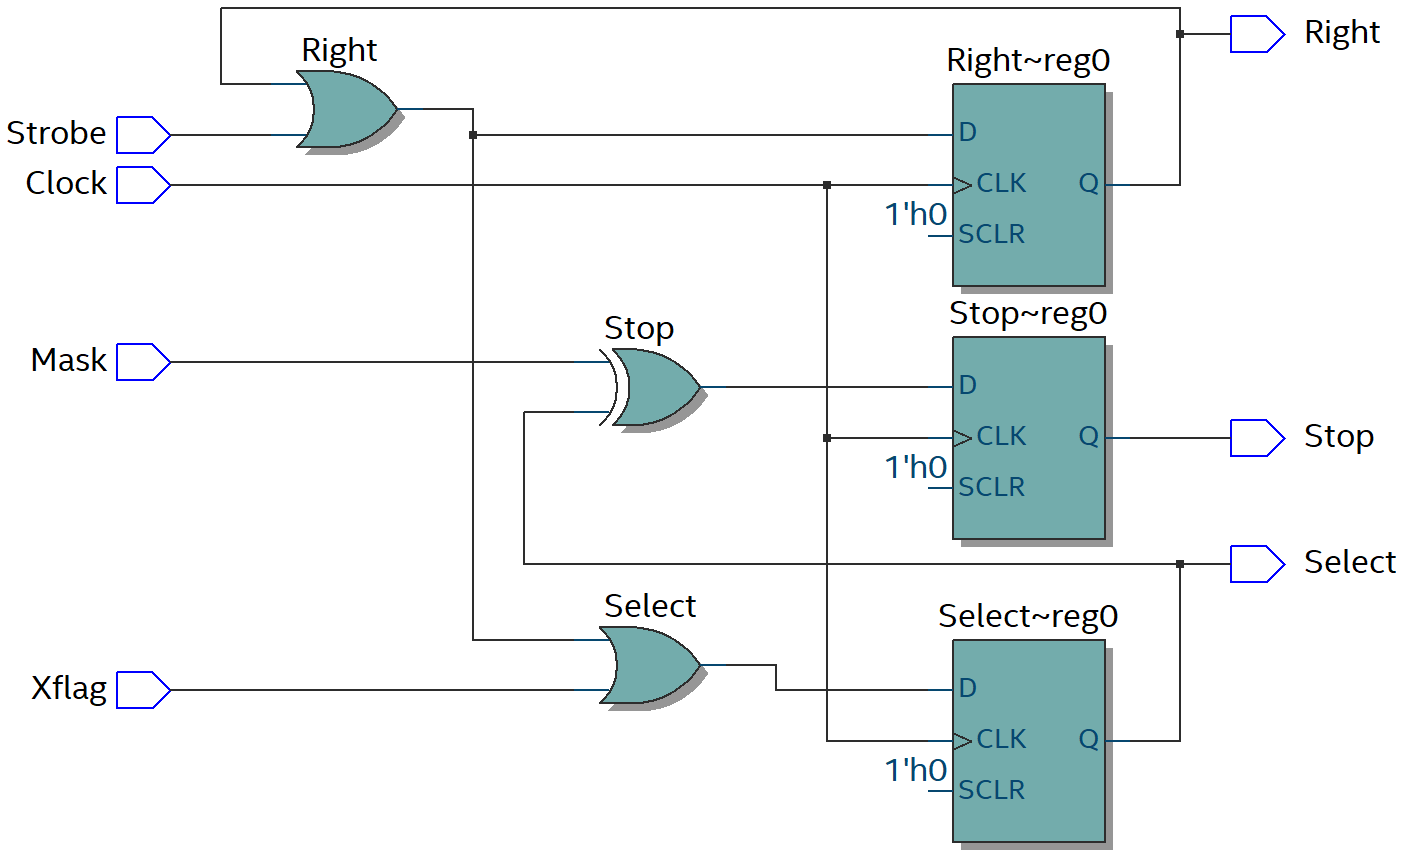
\includegraphics[scale=0.45]{Assignment_Circuit1_RTL.png}
	\caption{Diagrama RTL del circuito con múltiples asignaciones, descrito en Verilog. \label{fig:a_circuit1_rtl}}
\end{figure}

\begin{figure}[ht]
	\centering
	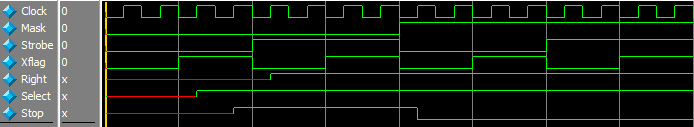
\includegraphics[scale=0.9]{Assignment_Circuit1_Wave.png}
	\caption{Simulación del circuito con múltiples asignaciones, descrito en Verilog, con el visor de formas de onda de ModelSim. \label{fig:a_circuit1_wave}}
\end{figure}